\documentclass{amsart}
\usepackage{amsmath, amssymb, amsthm}
\usepackage{tikz}

\theoremstyle{definition}
\newtheorem{problem}{Problem}
\theoremstyle{remark}
\newtheorem*{solution}{Solution}


\setcounter{problem}{0}


\title{Problems for 6.042 Spring 2013 final}
\author{Harry Sanabria}
\date{May 11, 2013}


\begin{document}

\maketitle

For Class Problem/Pset:
\begin{problem}
If $G_i$ is a $c_1$ colorable graph, and $G_2$ is a $c_2$ colorable graph on the same set of vertices, show that their union is $c_1*c_2$ colorable.
\end{problem}
\setcounter{problem}{0}

For the final:
\begin{problem}
Let $G_1$ and $G_2$ be two $k$-colorable graphs on the same set of vertices, and let $G$ be their union.  Show that we get a valid coloring for $G$ if we assign to each vertex a color based on the combination of two colors it has in $G_1$, $G_2$.  

For example, if $k=2$, and we color $G_1$ with colors 1, 2 and $G_2$ with colors A, B, then G will be colored with colors A1, A2, B1, B2, assigning to each vertex the combination of the two colors in the two subgraphs.

Conclude that $G$ is $k*k$-colorable.
\end{problem}

\begin{problem}
The chromatic number of a graph is the minimum number of colors needed to color the entire graph.  Find the chromatic number for the following graphs:
\end{problem}
a)
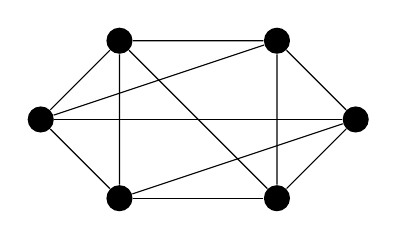
\begin{tikzpicture}
  [scale=.1,auto=left,every node/.style={circle,fill=black!100}]
  \node (n1) at (20,0) {};
  \node (n2) at (40,0) {};
  \node (n3) at (50,10) {};
  \node (n4) at (40, 20) {};
  \node (n5) at (20, 20) {};
  \node (n6) at (10, 10) {};

  \foreach \from/\to in {n6/n5,n5/n4,n4/n3,n3/n2,n2/n1,n1/n6,n1/n5,n1/n3,n2/n5,n2/n4,n3/n6,n4/n6}
    \draw (\from) -- (\to);
\end{tikzpicture}
b)
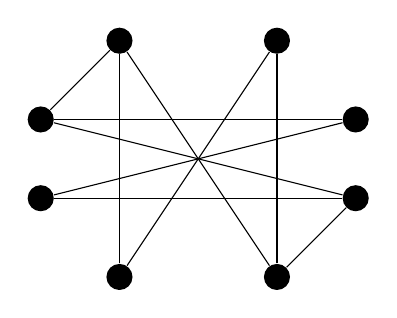
\begin{tikzpicture}
  [scale=.1,auto=left,every node/.style={circle,fill=black!100}]
  \node (n1) at (20,0) {};
  \node (n2) at (40,0) {};
  \node (n3) at (50,10) {};
  \node (n4) at (50, 20) {};
  \node (n5) at (40, 30) {};
  \node (n6) at (20, 30) {};
  \node (n7) at (10, 20) {};
  \node (n8) at (10, 10) {};

  \foreach \from/\to in {n1/n6,n1/n5,n2/n6,n2/n5,n2/n3,n3/n8,n3/n7,n4/n8,n4/n7,n6/n7}
    \draw (\from) -- (\to);
\end{tikzpicture}

\begin{problem}
a) Show that the relation $R$ such that: 
\[
u\ R\ v\ \text{$iff$ $u$ and $v$ are in the same connected component}
\]
is an equivalence relation.

b) Let $u,v$ be vertices of a simple, $n$-vertex graph.  Show that if $u$ and $v$ both have degree $\geq n/2$, then $u$ and $v$ are connected.  ($You\ can\ do\ part\ b\ without\ having\ done\ part\ a.$)
\end{problem}

\newpage
Solutions:
\setcounter{problem}{0}
\begin{problem}
\end{problem}
Class problem style:
For each vertex $v$ in $G$, color it with a new color defined by the combination of its two colors in $G_1$, $G_2$, such that each combination of colors is its own different color.  Clearly we will have $c_1 * c_2$ colors since there are that many combinations of the colors from each coloring.  

Now let's prove that this is a valid coloring.  Let $u,v$ be two vertices in $G$ such that there is an edge between them.  Since $G$ is the union of $G_1$, $G_2$, the edge between $u,v$ must be in either $G_1$ or $G_2$ (or both), so $u,v$ must have different colors in at least one of the two subgraphs.  Therefore, the combination of two colors in $u$ must differ from the combination of two colors in $v$ by at least one color, and therefore $u,v$ will have different colors in $G$.
\newline
\newline
Final Exam Style:
Let $u,v$ be two vertices in $G$ such that there is an edge between them.  Since $G$ is the union of $G_1$, $G_2$, the edge between $u,v$ must be in either $G_1$ or $G_2$ (or both), so $u,v$ must have different colors in at least one of the two subgraphs.  Therefore, the combination of two colors in $u$ must differ from the combination of two colors in $v$ by at least one color, and therefore $u,v$ will have different colors in $G$.

There are clearly $k*k$ combinations of two colors possible, so we can conclude that $G$ is $k*k$-colorable.

\begin{problem}
\end{problem}
a) 3-colorable with colors A, B, C. Cannot do better because there are triangles.
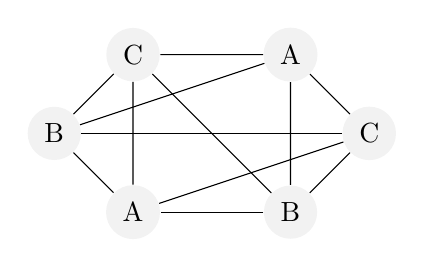
\begin{tikzpicture}
  [scale=.1,auto=left,every node/.style={circle,fill=gray!10}]
  \node (n1) at (20,0) {A};
  \node (n2) at (40,0) {B};
  \node (n3) at (50,10) {C};
  \node (n4) at (40, 20) {A};
  \node (n5) at (20, 20) {C};
  \node (n6) at (10, 10) {B};

  \foreach \from/\to in {n6/n5,n5/n4,n4/n3,n3/n2,n2/n1,n1/n6,n1/n5,n1/n3,n2/n5,n2/n4,n3/n6,n4/n6}
    \draw (\from) -- (\to);
\end{tikzpicture}


b) 2-colorable with colors A, B.
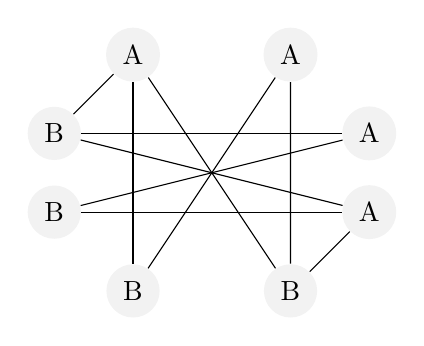
\begin{tikzpicture}
  [scale=.1,auto=left,every node/.style={circle,fill=gray!10}]
  \node (n1) at (20,0) {B};
  \node (n2) at (40,0) {B};
  \node (n3) at (50,10) {A};
  \node (n4) at (50, 20) {A};
  \node (n5) at (40, 30) {A};
  \node (n6) at (20, 30) {A};
  \node (n7) at (10, 20) {B};
  \node (n8) at (10, 10) {B};

  \foreach \from/\to in {n1/n6,n1/n5,n2/n6,n2/n5,n2/n3,n3/n8,n3/n7,n4/n8,n4/n7,n6/n7}
    \draw (\from) -- (\to);
\end{tikzpicture}

\begin{problem}
\end{problem}
a) We show that $R$ is reflexive, symmetruc, and transitive.

reflexive: $v$ is always in the same connected component as itself, so $vRv$ holds.

symmetric: if $uRv$ holds, $u,v$ are in the same connected component, so $vRu$ also holds.

transitive: if $uRv$ and $vRw$ hold, then trivially $u,v,w$ are all in the same connected component and therefore $uRw$ holds.
\newline
\newline
b) Proof by contradiction:

Let us assume, for the sake of contradiction, that $u,v$ are not connected. Define:
\[
U:==\{ w | \text{there is an edge from $u$ to $w$}\}
\]
\[
V:==\{ w | \text{there is an edge from $v$ to $w$}\}
\]
Then since $u,v$ are not connected, $u$ is not in $V$ and $v$ is not in $U$.  Additionally, $U$ and $V$ must share no elements in common.  $|U|=|V|=n/2$, which means that for $U$ and $V$ to share no elements in common, $|U\cup V|=n$, meaning they must contain $n$ vertices in total.  However, since $u,v$ is in neither set, there are only $n-2$ vertices remaining in the graph to chose from, and we have reached a contradiction.  Therefore, $U,V$ must share an element and therefore $u,v$ are connected.







\end{document}
